\chapter{Desenvolvimento}
\label{chap:fundteor}

Neste capítulo serão demonstrados os desafios e trabalhos realizados durante o programa de formação em Robótica e Sistemas Autônomos.

%--------- NEW SECTION ----------------------
\section{Desafio 1.0 - Simulação do ambiente externo do CIMATEC 4}
\label{sec:des1}

Este desafio foi realizado de maneira individual, e consiste na simulação de um robô UGV (\textit{Unmanned Ground Vehicle}) da \textit{Clearpath Robotics} chamado \textit{Husky} (Figura \ref{img:des1husky}), no ambiente simulado \textit{Gazebo}. O ambiente de trabalho é uma representação em 3D \textit{CAD (Computer Aided Design)} da área externa do CIMATEC 4 (Figura \ref{img:des1mapreal}), como visto na Figura \ref{img:des1map}. Sua missão era achar uma bola amarela de 1 metro de raio (Figura \ref{img:des1ball}) que possuía localização aleatória no ambiente de trabalho. Durante a missão, o robô deve navegar autonomamente e realizar a detecção da bola via câmera. O objetivo da missão era concluído quando o robô se aproximasse até 1 metro da bola e enviasse uma mensagem de conclusão.

%---------------picture------------------------------------
\begin{figure} [H]												
    \centering
    \caption{Vista superior da área externa do CIMATEC 4.}
	\includegraphics[width=1.0\textwidth]{./des1mapreal}	
	\caption*{Fonte: \textit{Google Earth}}		
	\label{img:des1mapreal}									 
\end{figure}												

\begin{figure} [H]												
    \centering	
    \caption{Representação em \textit{CAD} utilizando o \textit{software OnShape}.}								
	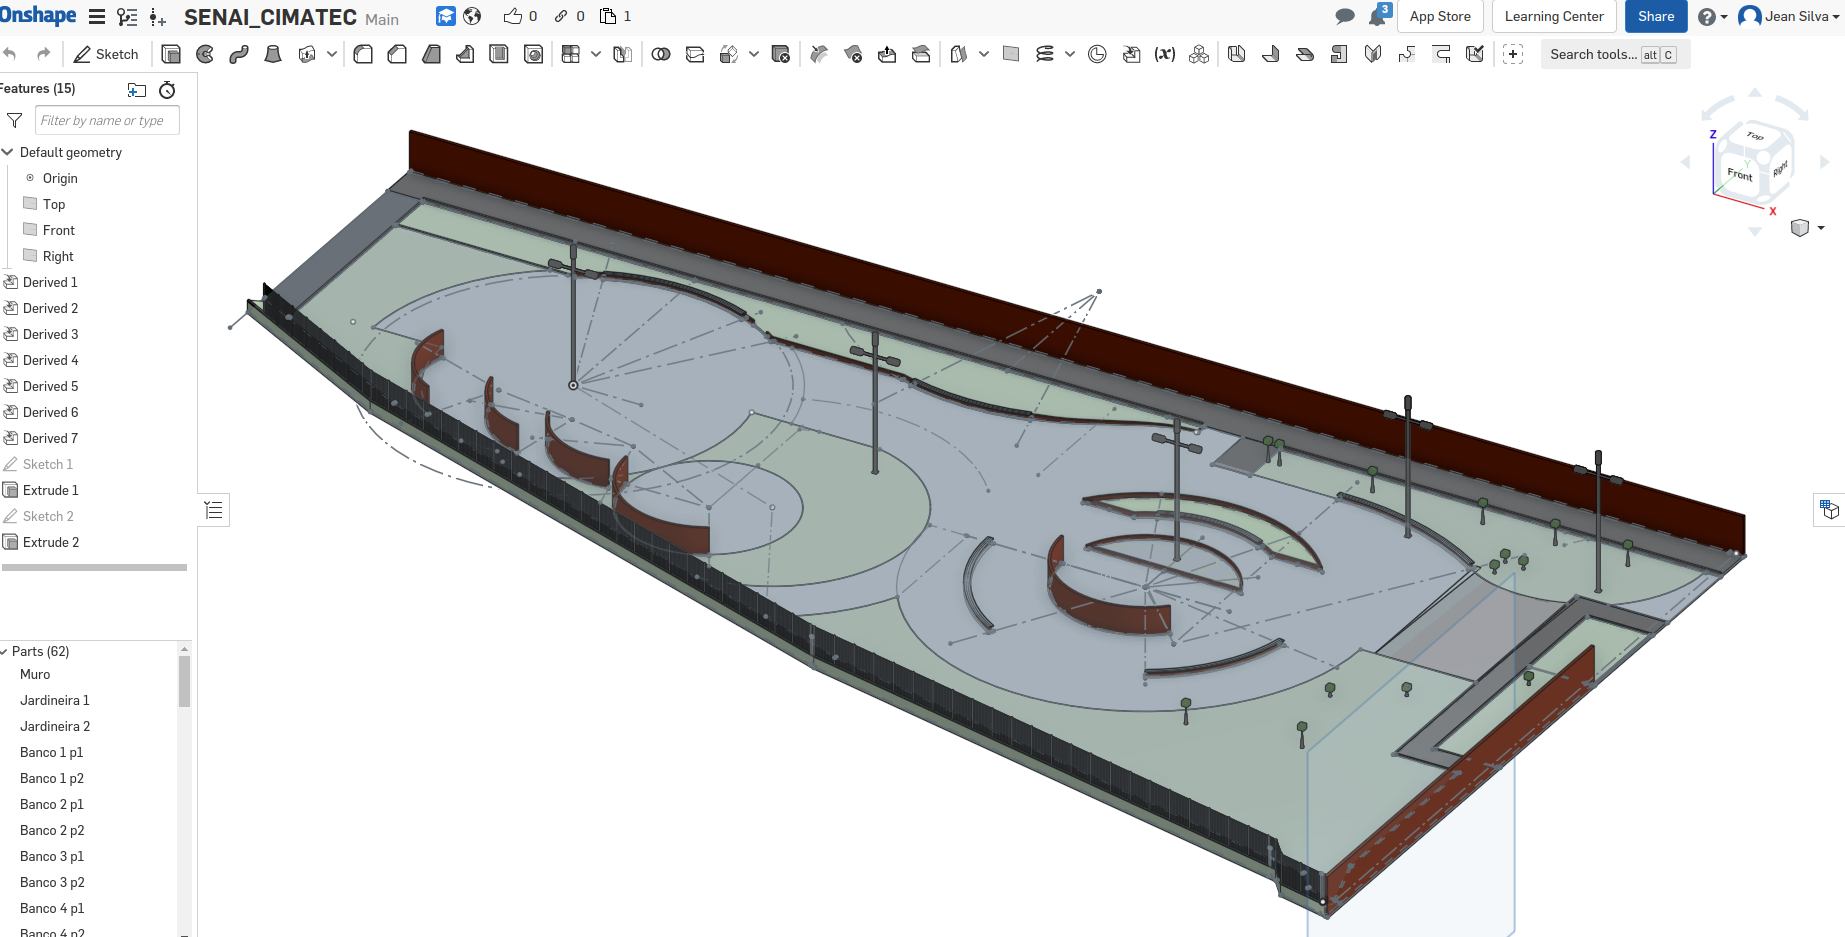
\includegraphics[width=1.0\textwidth]{./des1map}	
	\caption*{Fonte: Grupo de formação em Robótica e Sistemas Autônomos}		
	\label{img:des1map}									 
\end{figure}

\begin{figure} [H]												
    \centering
    \caption{Robô \textit{Clearpath Husky} simulado em ambiente \textit{Gazebo}.}										
	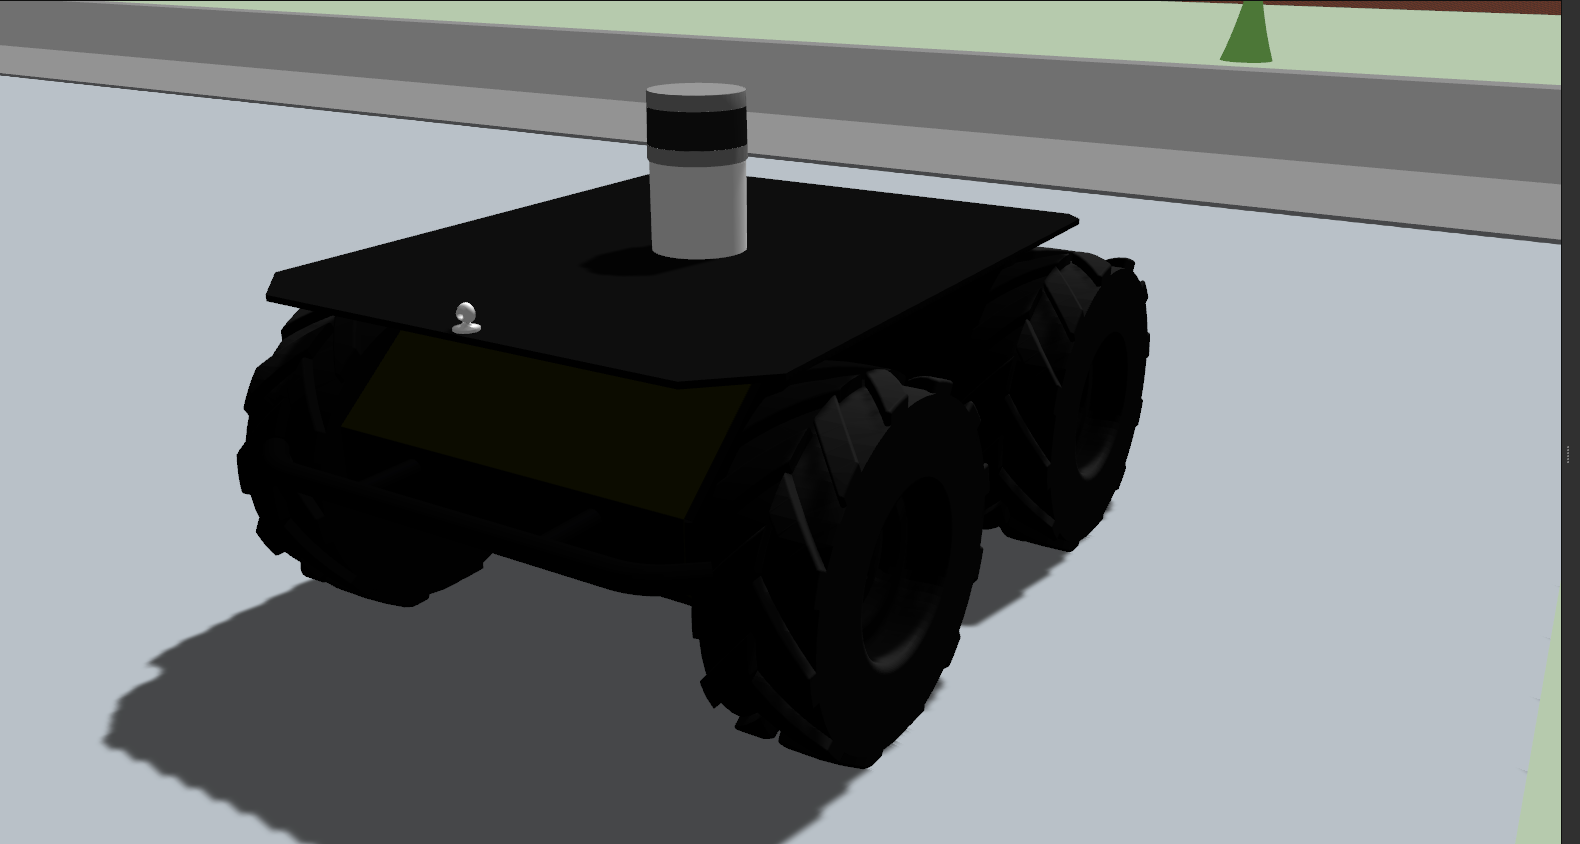
\includegraphics[width=1.0\textwidth]{./des1husky}	
	\caption*{Fonte: Grupo de formação em Robótica e Sistemas Autônomos}		
	\label{img:des1husky}									 
\end{figure}

\begin{figure} [H]												
    \centering
    \caption{Bola amarela no ambiente de trabalho simulado.}												
	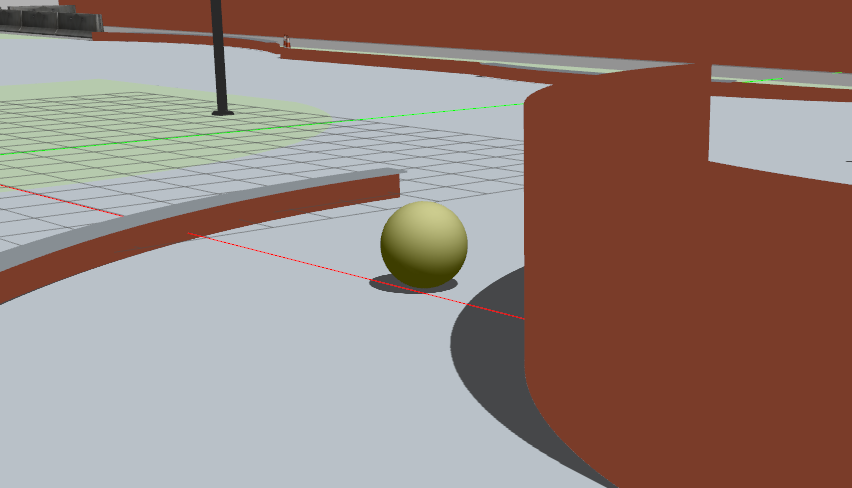
\includegraphics[width=1.0\textwidth]{./des1ball}	
	\caption*{Fonte: Grupo de formação em Robótica e Sistemas Autônomos}
	\label{img:des1ball}									 
\end{figure}
%----------------------------------------------------------

%--------- NEW SECTION ----------------------
\section{Desafio 2.0 - Entrega parcial: simulação do manipulador robótico RAJA}
\label{sec:des2}

Este desafio foi realizado em grupo de 4 pessoas e consistiu na simulação em \textit{Gazebo} de um manipulador robótico com 5 graus de liberdade de nome RAJA. Ele possui uma câmera \textit{RGB (Red, Green and Blue)} que tem finalidade em encontrar a posição de um botão de uma caixa no seu ambiente de trabalho. Esta posição é definida por um marcador fiducial \textit{ArUco (Augmented Reality by University of Cordoba)} que a caixa possui. Com a posição encontrada, o manipulador pressiona o botão com sua ferramenta. Todos os modelos simulados foram feitos no \textit{OnShape}. A Figura \ref{img:des2} representa o manipulador em seu ambiente de trabalho ao chegar até o botão. O Apêndice \ref{append:raja} representa o relatório deste desafio com suas especificações, arquitetura, desenvolvimento, metodologia e resultados.

\begin{figure} [H]												
    \centering
    \caption{Manipulador RAJA finalizando a missão.}	
	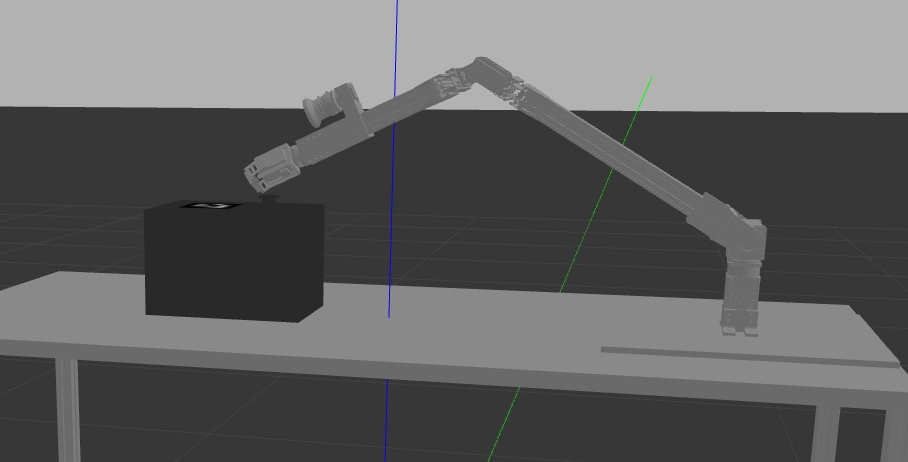
\includegraphics[width=1.0\textwidth]{./des2}	
	\caption*{Fonte: Grupo de formação em Robótica e Sistemas Autônomos}
	\label{img:des2}									 
\end{figure}

%--------- NEW SECTION ----------------------
\section{Desafio 2.2 - Entrega final do manipulador JeRoTIMON}
\label{sec:des22}

Este desafio realizado em um grupo de 6 pessoas, visou construir um modelo físico de um manipulador robótico baseado nos conceitos aplicados no desafio 2.0 (Subseção \ref{sec:des2}). Os objetivos continuaram os mesmos: obter a posição de um botão em uma caixa baseado em um marcador fiducial \textit{ArUco} utilizando uma câmera \textit{RGB} modelo \textit{Teledyne Genie Nano C2590} e pressioná-lo utilizando o manipulador robótico. A construção física do manipulador foi realizada com os materiais disponíveis no laboratório de Robótica e Sistemas Autônomos do SENAI CIMATEC. Sua base foi feita de madeira com suportes de aço, e os elos foram feitos com alumínio. Os motores são de marca ROBOTIS e modelos Dynamixel PLUS. A peça de suporte para a câmera foi feita a partir de impressão 3D com material ABS. A Figura \ref{img:des22} mostra o manipulador em seu ambiente de trabalho com a caixa objetivo. No Apêndice \ref{append:jerotimon} está disponível o relatório com maiores detalhes sobre o desenvolvimento, metodologia e resultados.

\begin{figure} [H]												
    \centering
    \caption{Manipulador JeRoTIMON no ambiente de trabalho e a caixa objetivo.}	
	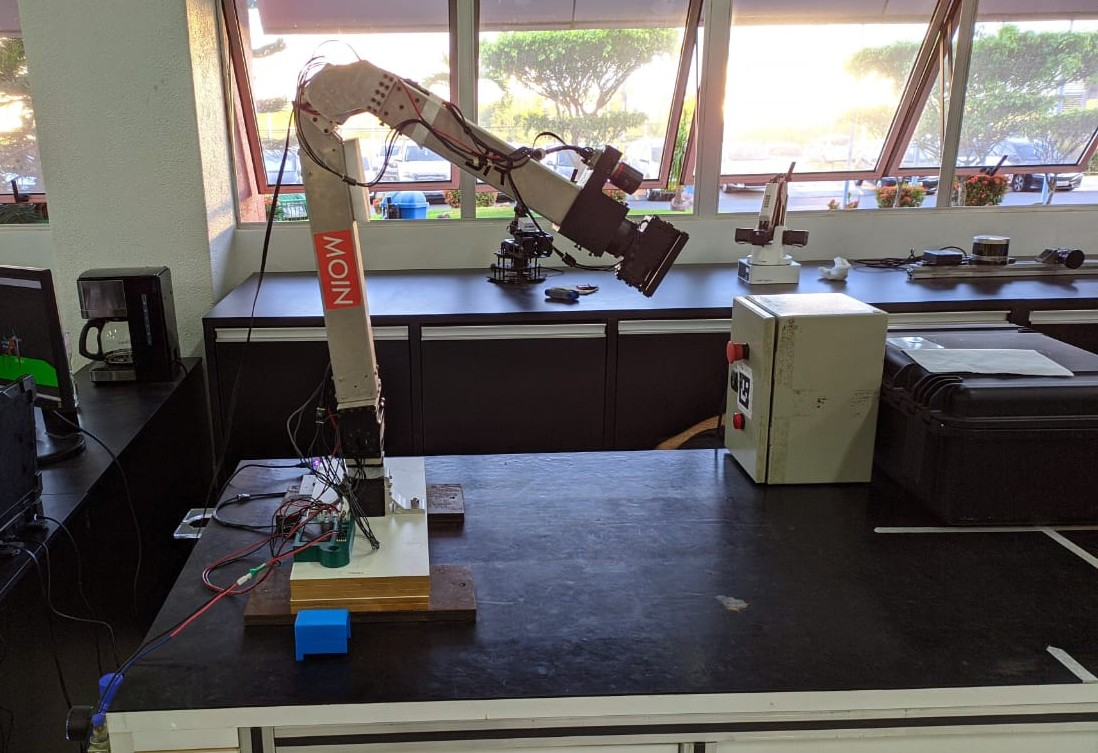
\includegraphics[width=1.0\textwidth]{./des22}	
	\caption*{Fonte: Grupo de formação em Robótica e Sistemas Autônomos}
	\label{img:des22}									 
\end{figure}


%--------- NEW SECTION ----------------------
\section{Desafio 2.5 - Análise estatística R\&R do robô Darwin-OP}
\label{sec:des25}

Este desafio foi realizado em um grupo de 4 pessoas, as mesmas do desafio \ref{sec:des2}. O objetivo deste trabalho era desenvolver um ambiente simulado em \textit{Gazebo}, e realizar ações autônomas de marcha liderada e corrida de revezamento com 4 robôs humanóides \textit{Darwin-OP} (Figura \ref{img:darwin}). Na marcha liderada, os 4 robôs devem andar em velocidade sincronizada durante 2 metros, como mostra a Figura \ref{img:marcha}. Na corrida de revezamento, cada robô está posicionado em uma parte específica da pista de corrida (Figura \ref{img:revezamento}), em que ele deve aguardar o robô anterior se aproximar, manter-se próximo em velocidade sincronizada por cerca de 5 segundos (representando a passagem de bastões) e depois seguir em maior velocidade para alcançar o robô à sua frente. A pista projetada pode ser visualizada na Figura \ref{img:pista}.

Este projeto teve um estudo estatístico que pode ser visto no Apêndice \ref{append:darwin}, e tem por objetivo analisar a medição dos dados utilizando o método de análise de variância.

\begin{figure} [H]												
    \centering
    \caption{\textit{Darwin-OP} em ambiente simulado.}	
	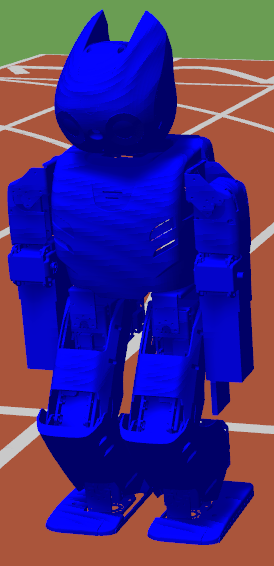
\includegraphics[width=0.6\textwidth]{./darwin-op}	
	\caption*{Fonte: Grupo de formação em Robótica e Sistemas Autônomos}
	\label{img:darwin}									 
\end{figure}

\begin{figure} [H]												
    \centering
    \caption{\textit{Darwin-OP} em posição de marcha liderada.}	
	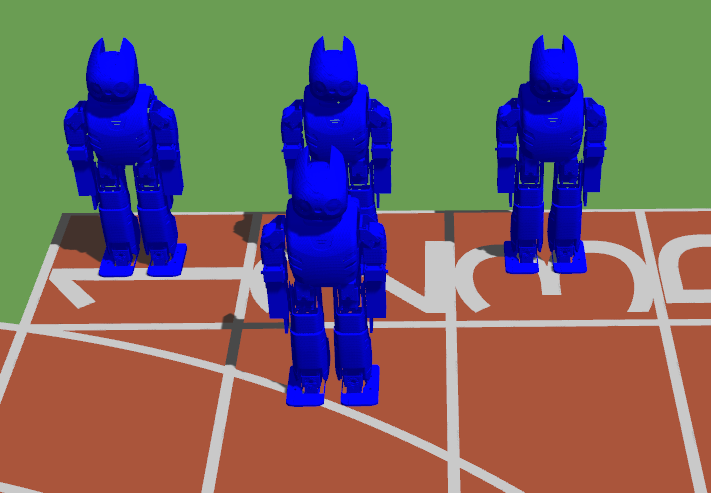
\includegraphics[width=1.0\textwidth]{./ordunmarcha}	
	\caption*{Fonte: Grupo de formação em Robótica e Sistemas Autônomos}
	\label{img:marcha}									 
\end{figure}

\begin{figure} [H]												
    \centering
    \caption{\textit{Darwin-OP} em posição de revezamento.}	
	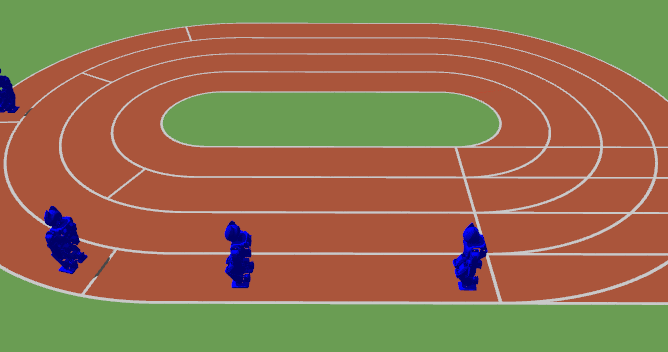
\includegraphics[width=1.0\textwidth]{./visao-darwin}	
	\caption*{Fonte: Grupo de formação em Robótica e Sistemas Autônomos}
	\label{img:revezamento}									 
\end{figure}

\begin{figure} [H]												
    \centering
    \caption{Pista e suas dimensões.}	
	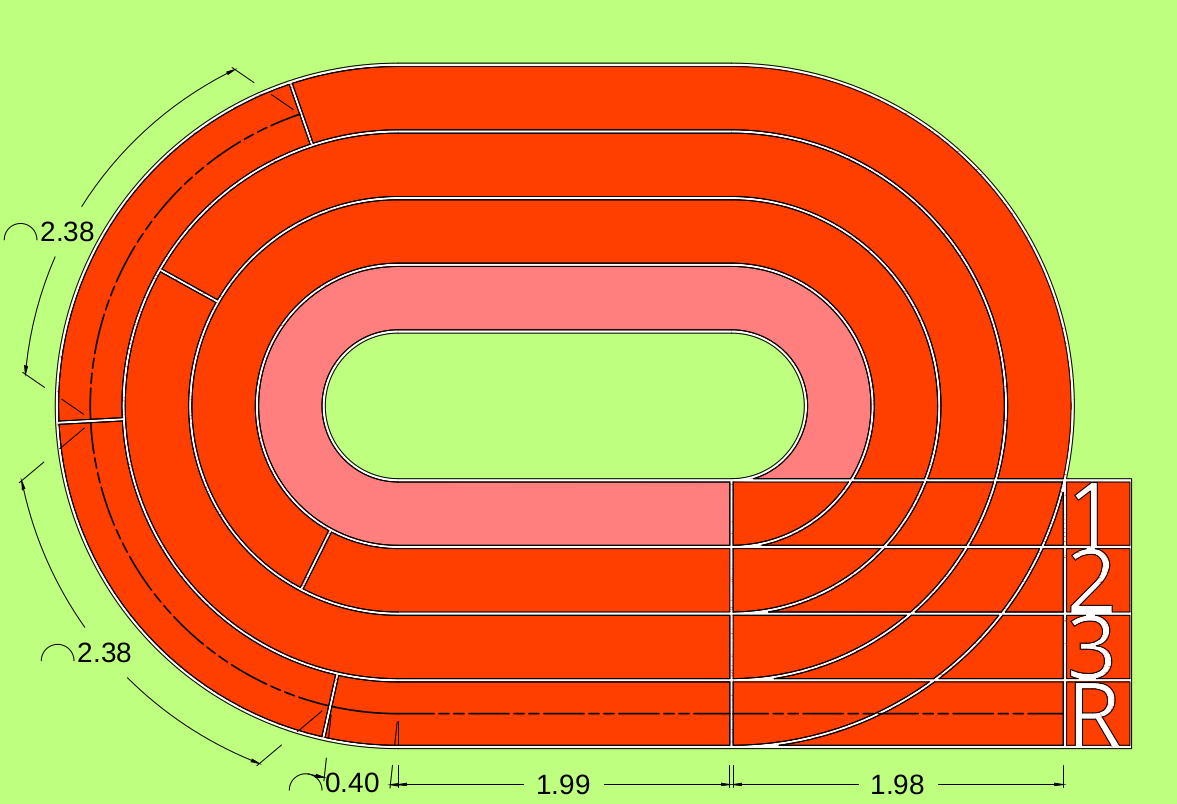
\includegraphics[width=1.0\textwidth]{./track}	
	\caption*{Fonte: Grupo de formação em Robótica e Sistemas Autônomos}
	\label{img:pista}									 
\end{figure}

%--------- NEW SECTION ----------------------
\section{Desafio 3.0 - Curupira}
\label{sec:des3}

Este desafio foi realizado por um grupo de 3 pessoas. O projeto Curupira representa a integração do \textit{UGV Clearpath Robotics Warthog} e o manipulador JeRoTIMON, visto na Subseção \ref{sec:des22}. Equipado com sensores para as funcionalidades de percepção de localização, como câmera \textit{RGB}, \textit{LIDAR (Light Detection and Ranging)} e \textit{GPS (Global Positioning System)}, o objetivo é dar autonomia ao sistema para que ele consiga identificar uma ``bomba'' (Figura \ref{img:bomba}) presente em um lugar aleatório da área externa ao CIMATEC 4 (visto na Figura \ref{img:des1mapreal} na Subseção \ref{sec:des1}). A posição do objetivo é adquirida pela câmera, e o objetivo é considerado completo quando o manipulador tocar nos fios da ``bomba''.

Este projeto foi dividido em duas partes: simulada em ambiente \textit{Gazebo}; e a construção real da integração, visto na Figura \ref{img:curupira}. O desenvolvimento, metodologia e resultados podem ser vistos no Apêndice \ref{append:curupira}.

\begin{figure} [H]												
    \centering
    \caption{``Bomba'' identificada pela rede neural no ambiente de trabalho.}	
	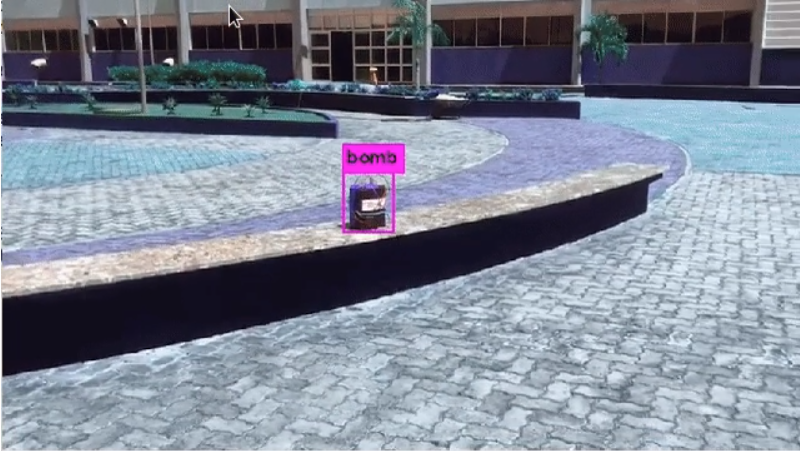
\includegraphics[width=0.8\textwidth]{./int-detection2}	
	\caption*{Fonte: Grupo de formação em Robótica e Sistemas Autônomos}
	\label{img:bomba}									 
\end{figure}

\begin{figure} [H]												
    \centering
    \caption{Integração física.}	
	\includegraphics[width=0.55\textwidth]{./modularidade}	
	\caption*{Fonte: Grupo de formação em Robótica e Sistemas Autônomos}
	\label{img:curupira}									 
\end{figure}

%--------- NEW SECTION ----------------------
\section{Estudo estatístico de \textit{DOE (Design of Experiments)}}
\label{sec:doe}

Este desafio foi realizado em um grupo de 4 pessoas, as mesmas do desafio \ref{sec:des2}. O objetivo deste experimento foi aplicar os conceitos de estatística aprendidos durante a especialização. Foi utilizado um modelo de helicóptero de papel em um experimento de medição do seu tempo de queda. Durante o processo de medição, foram adicionados adesivos e clipes ao helicóptero, modificando seu tempo de queda. Os conceitos de \textit{DOE} foram aplicados para identificar quais os fatores mais influenciam a variável controlada: tempo de vôo. Esta análise foi feita utilizando o \textit{software} estatístico \textit{R Studio} para tratamento dos dados e visualização final. Os resultados e interpretações estão no Apêndice \ref{append:doe}.